

\documentclass[12pt,a4paper]{book}



			% Packages Files
%----------------------------------%

	% Page Setttings
\usepackage[top = 1in, bottom = 1in, left = 1in, right = 1in]{geometry}

\parindent=0cm % to prevent the spacing in new paragraph or new line

\usepackage{fancyhdr} % needded for header and footer 

%-----------------------------------------------------------------%

\usepackage{amsmath} % needed for referencing thequation
\usepackage{amsfonts} % for maths symbols
\usepackage{graphicx}
\usepackage[export]{adjustbox}
\usepackage{caption}
\usepackage{refstyle} % to reference a captioned figure


% To make hyperlinks

\usepackage[
	colorlinks=true
	,breaklinks
	]{hyperref} % needed for creating hyperlinks in the document, the option colorlinks=true gets rid of the awful boxes, breaklinks breaks lonkg links (list of figures),
	
\usepackage{xcolor}
\definecolor{c1}{rgb}{0,0,1} % blue
\definecolor{c2}{rgb}{0,0.3,0.9} % light blue
\definecolor{c3}{rgb}{0.3,0,0.9} % red blue
\hypersetup{
    linkcolor={c1}, % internal links
    citecolor={c2}, % citations
    urlcolor={c3} % external links/urls
}

	% For Code Writing
	
\usepackage{listings}

\usepackage{color}

\definecolor{mygreen}{rgb}{0 0.6 0}

\lstset{
% Set automatic Line breaking, in case we have long lines don't
% fit inside the frame or the page.
breaklines = true,
commentstyle = \color{mygreen},
breakatwhitespace = true,% don't show white space character
%numbers = left, % put line number in the code
keywordstyle=\color{blue}
title = \lstname
}

% ------------- For Writing Equations inisde a table and centering them ------------

\usepackage{array}

% Vertical Alignment inside the cells of the table
\newcolumntype{M}[1]{>{\centering\arraybackslash}m{#1}}

% Horizontal Alignment inside the cells of the table
\newcolumntype{P}[1]{>{\centering\arraybackslash}p{#1}}

% Wrting list inside a table

% \usepackage[shortlabels]{enumitem}
 
% \usepackage[shortlabels]{enumitem}

% -------- Multi Row Table------------
\usepackage{multirow}

% %---------- needed for long tables over pages-------
\usepackage{longtable} 


\usepackage{subfig}
% To adjust the page style
\usepackage{fancyhdr}


% needed for todos liste
\usepackage{todonotes} 


% ----------------- Tikz Package --------------

\usepackage{tikz}

\usetikzlibrary{shapes,shadows,arrows}

\usetikzlibrary{calc}






% Macros File

% Macros Example
\def\labelaxes{Remember to include some suitable labeling for the axes and the units used in measurements.}

% 2nd way for defnining macros: the new command
% 1st parameter: name of the new command
% 2nd paramter: how many inputs this command needs, in this case only 1
% 3rd parameter: what this new command named \tbi do

\newcommand{\tbi}[1]{\textbf{\textit{#1}}}

% Command for Picture without a label

\newcommand{\pic}[3]{\begin{figure}[h]
\centering
\includegraphics[width = 0.7\textwidth, frame]{#1}
\caption{#2}
\end{figure}}








\DeclareMathOperator*{\argmax}{argmax} % thin space, limits underneath in displays

\DeclareMathOperator*{\argmin}{argmin}

\title{System Programming in C}
\author{Ranim Tom}



\begin{document}

% downloaded template
%\input{content/title_page_1} 

%\maketitle
\tableofcontents


% to make the todo list appear as a table of content
\listoftodos

\pagestyle{fancy}
\fancyhf{} % Clear header and footer
\rhead{\rightmark}
\lhead{Chapter \thechapter}
\rfoot{Page \thepage}

\chapter*{Abstract}

The goal of this reader is to summarize my learning in system programming in \verb|C|.

\chapter{Introduction}

\section{System programming concepts}

\begin{itemize}

\item purpose for user mode: user application software must prevent to access the hardware directly, because it could damage the hardware.

Hence the kernel provide a layer between the user application and the hardware.

\item If a user program needs to access hardware,  it will be done via the kernel mode

    \begin{itemize}
        \item In this mode, we have a set of calls and programs to access the hardware

        \item Once the required information is fetched from the hardware,  it will be passed to user application
    \end{itemize}

\item What is  a kernel?

The kernel is the core of an OS, which handles resources.

It resides inside the memory, and it is the $\mathrm{1}^\mathrm{st}$ thing that comes at the start of a bootloader


\item Function of a kernel

    \begin{itemize}
    
    \item file management

    \item  memory management: making the memory available to different processes via the virtual memory management


    \item Interprocess communication: how different processes communicate with each other

    \item Threads (so multitasking system)
    \end{itemize}


\item Linux as layer view

\begin{itemize}
    \item Linux hide hardware from direct access by user application, because if so it can damage the hardware

    \item \todo{Linux layer} \textit{Linux layer: to insert a picture later}
\end{itemize}

\item When accessing hardware, the OS turns into kernel mode

    \begin{itemize}
        \item \todo{kernel mode} \textit{kernel mode: to see if this is called also privilege mode}
    \end{itemize}

\end{itemize}


\todo{kernel function} \textit{kernel functions and concept}

\begin{itemize}

\item \textit{to define and write later different new concept used, like what is a process, a  thread, concepts about Linux OS, $\cdots$}

\item \textit{Add references about system programming later}

\end{itemize}


\newpage
\section{System Call}


\subsection{Library}

Before diving into system call, let's fix the terminology first.

In a normal \verb|C| program, we need to include \tbi{header files} to use some function, such as \verb|stdio.h| to use \verb|printf()|.
This type of library is called \tbi{C standard library}.\\

\subsection{Getting into system call}

Now in system programming, we have some libraries which are designed to operate in a system call.\\

So what is a system call?\\

System calls (often shortened to \textit{syscalls}) are function invocations made from user space—your text editor, favorite game, and so on—into the kernel (the core internals of the system) in order to request some service or resource from the operating system (chapter 1 in \cite{book_Linux_System_Programming_Robert_Love}) 



\begin{itemize}

\item  The programs run in a kernel mode during system call execution

\item There are 2 ways to perform system call:

\begin{itemize}
    \item Or using directly the kernel like the function \verb|write()|
    
    \item Through a library function.

    Example is \verb|prinf()| which in turns call \verb|write()|

\end{itemize}

\end{itemize}

\newpage
\subsection{Internal mechanism for system call}

\begin{itemize}
    
\item The functional block diagram is shown in \autoref{fig:concept_system_programming:sys_call_diagram}.

\begin{figure}[h]
\centering
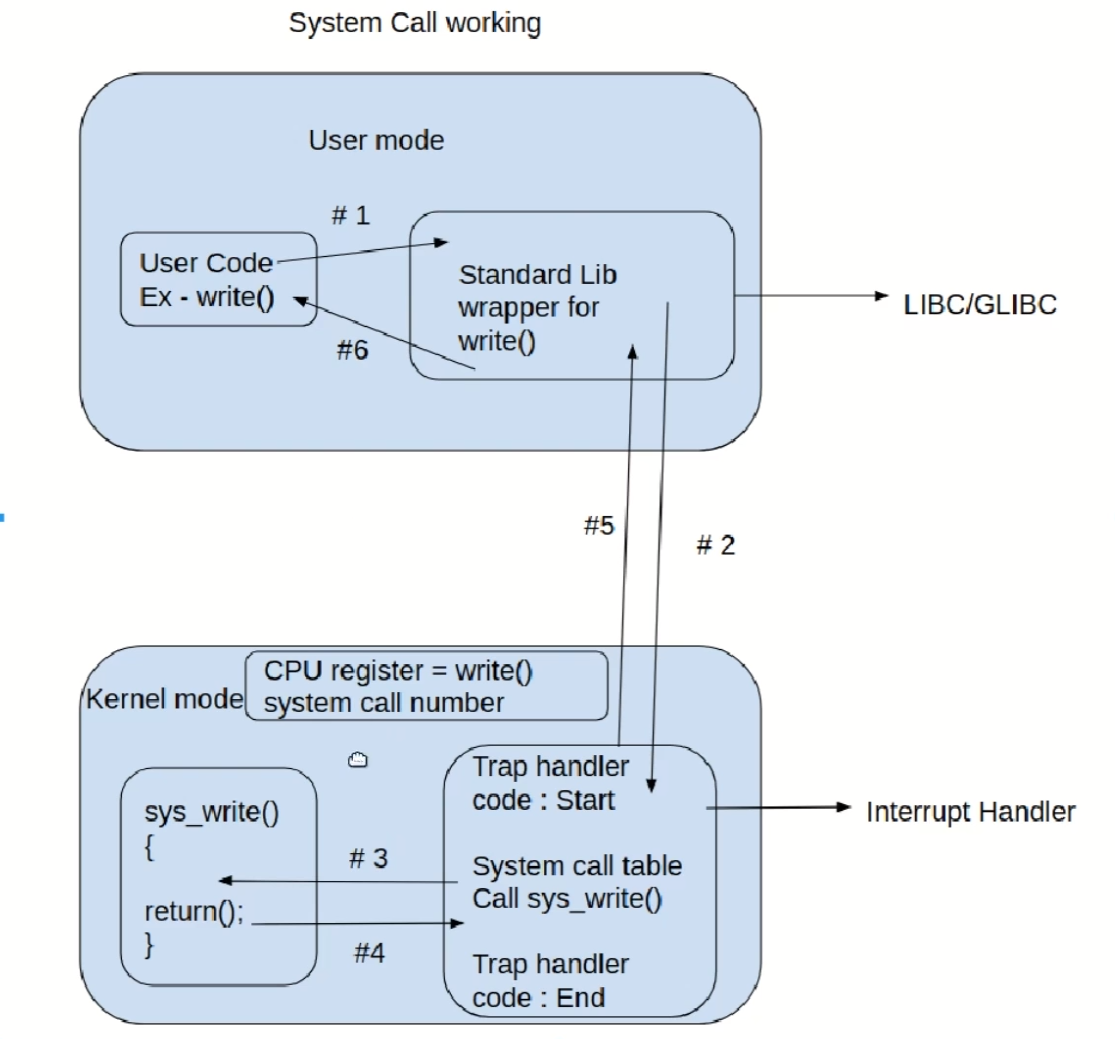
\includegraphics[width = 0.7\textwidth, frame]{Figures/concept_system_programming/sys_call_diagram}
\caption{Main Components}
\label{fig:concept_system_programming:sys_call_diagram}
\end{figure}


\item Every system call has a unique number associated with it 


\item When we use \verb|write()| function in our code, it will no directly invoke the definition (implementation), rather it will call a \tbi{wrapper}

\item This wrapper will raise an interrupt specific to hardware, and will compare the number associated to this function, in order to search to system call actual definition

\item Finally we will get to the actual function and get back the outputs

\item  Then we turn our way up to the user space again with the correct output.

\end{itemize}


\chapter{File I/O}

\section{Introduction}

Now we move for file manipulation in system programming.

Files are important in linux system programming, because everything is a treated as file in linux (chapter in 1 in \cite{book_Linux_System_Programming_Robert_Love}).\\


\underline{Under the hood info:}

\begin{itemize}
    \item Once we open a file, a metadata is attached to this open state is called file descriptor, known as \verb|ftd|, which is handled as \verb|int| \verb|C| type.
\end{itemize}


\section{File types}

There exist many file types in system programming, as shown in \autoref{fig:files:file_types}.

\begin{figure}[h]
\centering
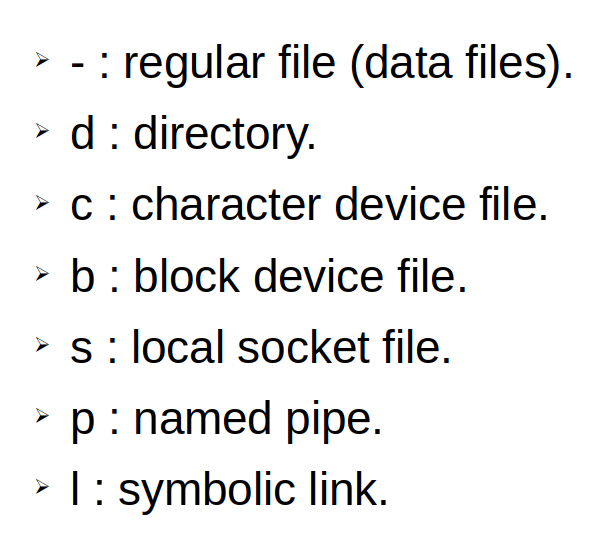
\includegraphics[width = 0.7\textwidth, frame]{Figures/files/file_types.png}
\caption{File types}
\label{fig:files:file_types}
\end{figure}



%====================================================
%====================================================
%====================================================

\chapter{Processes}

\section{References}

\begin{itemize}

\item chapter 5 in \cite{book_Linux_System_Programming_Robert_Love}

\item chapter 2 in \cite{book_modern_operating_system}

\end{itemize}

\section{Introduction}

Processes are next to files, the $\mathrm{2}^\mathrm{nd}$ important abstraction unit in Unix system.

In simple terms, we can define a process a program being executed such as \verb|C| program.

But a process is also much bigger than that: it contains kernel resources, virtualized memory, many threads,$\cdots$.

Some concepts:

\begin{itemize}

\item a process is an exected program (such as a build \verb|C| program)

\end{itemize}

\todo{Process Intro} \textit{Process Intro}

\begin{itemize}

\item \textit{To read later from books about processes, and the youtube videos I saw before}

\item \textit{To see the youtube playlist about processes}

\end{itemize}

\underline{youtube playlist}

\begin{itemize}

\item \url{https://www.youtube.com/watch?v=OrM7nZcxXZU&list=PLBlnK6fEyqRgKl0MbI6kbI5ffNt7BF8Fn}

    \begin{itemize}
        \item Neso Academy for operating systems

        \item Can serve as theory and complementary explanation for my books reading
    \end{itemize}

\item  \url{https://www.youtube.com/watch?v=cex9XrZCU14&list=PLfqABt5AS4FkW5mOn2Tn9ZZLLDwA3kZUY}

    \begin{itemize}
        \item nice playliste for examples in \verb|C|

        \item Contains alos a playlist for threads
    \end{itemize}

\end{itemize}

\section{Process ID}

\newpage
\section{Process states}

Talk about the life cycle after the process is created (using the \verb|fork()| system call).

\newpage
\section{Process creation}

\underline{Important points of the video:} The following points are about the \verb|fork()| system call used to create processes in linux


\begin{itemize}

\item once \verb|fork()| is used to create the process, the child process will have the same resources as the parent process.

\item The special thing about \verb|fork()| is it returns value in 2 places:

    \begin{itemize}
        \item In the parent process, the process ID \verb|pid_t|

        \item In the child process, it returns -1 or error
        
    \end{itemize}

\item The child process execute the same program as the parent process

\item Each process can now modify their variables without affecting the other, and store in its correspondent memory segment (heap, stack,$\cdots$) 

\end{itemize}


In \autoref{fig:processes:fork_before_after}, we have the state of before and after. 

In other words, once we use the \verb|fork()| in some \verb|C| source file, starting from this line we have 2 branches (2 codes), each with a separate memory

\begin{figure}[h]
\centering
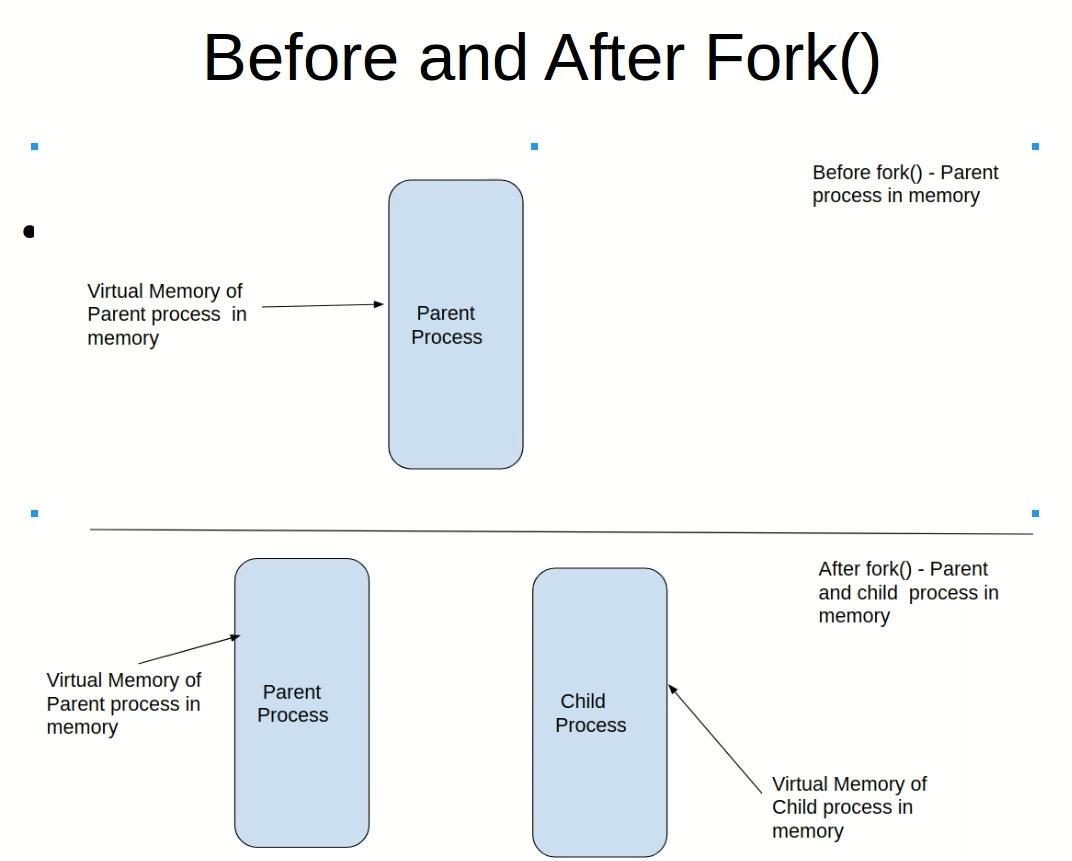
\includegraphics[width = 0.7\textwidth, frame]{Figures/processes/fork_before_after}
\caption{fork system call: before and after}
\label{fig:processes:fork_before_after}
\end{figure}

\subsection{Copy on- write}

We can see that in \autoref{fig:processes:fork_before_after} after \verb|fork()| is being called, that we have 2 memory section: once for each process. So we can say that the OS make a copy of the memory. This was the old style employed by Unix system.

Now in modern Unix system such as Linux, copy is note made  directly (to avoid unnecessary copy), and the 2 processes share the same memory. It is only when one of the processes need to alter or change some resources, copy will be made.

In other words, if one of the processes (parent or chlid) require some \tbi{modification of the data}, only then a separate memory will be duplicated.

Hence the name copy on write.\\

For further information about the mechanism, see chapter 5 in \cite{book_Linux_System_Programming_Robert_Love}.



\newpage
\section{Waiting a process}

\begin{itemize}

\item  Sometimes a process need to wait for the child process in order to terminate

\item  Each process which terminate has an exit status

\item terminating a process is done via the \verb|void exit(int status)|

    \begin{itemize}
        \item The important thing about this function is that it does not return anything to see if the a certain process is finished or not

        \item  We need to see the \verb|status| variable to know if the status has finished or not
    \end{itemize}

\end{itemize}

\todo{Video} \textit{Video course: video 38, at 20:17}.

\newpage
\section{Memory Layout}
Now we discuss memory layout for the process.

Memory a of process is composed of different \tbi{segments} as enumerated below

\begin{enumerate}

\item Text: code reside here

    \begin{itemize}
        \item that is the code of the program is being executed

        \item this segment is a \textit{read only} $\leftrightarrow$ can't be altered by any pointer
    \end{itemize}

\item Data: data variables during compile time

    \begin{itemize}
        \item It is composed between uninitialized and initialized data 
    \end{itemize}

\item  stack: for local variables and functions

    \begin{itemize}
        \item the composition inside the stack is called \textit{frame}

        \item each frame contains 1 functions and its related variables
    \end{itemize}

\item heap: dynamic variables

\end{enumerate}

\subsection{Code Example}

\todo{Code Example} \underline{\textit{Code Example:}}

\begin{itemize}

\item \textit{To do later some examples using some example programs}

\item \textit{To see video number 26 from the course, and examples from the books also}

\end{itemize}


\newpage
\section{Notes and summary}

\begin{itemize}

\item About the memory layout: a nice example about text segment and how it is read only, the code \verb|char* buff = "welcome"|.

    \begin{itemize}
        \item \verb|welcome| variable here is store in the text segment, so we can't change it

        \item If we try to do \verb|buff[0] = '\n'|, it will result in a segmentation fault
    \end{itemize}


\end{itemize}


\chapter{Virtual Memory}


\section{The big picture}

The virtual memory concept allow the process to access more address space then the actual physical RAM.

\textit{Concept to be reviewed later:}

\begin{itemize}

\item \textit{Concept of an address space}

\item \textit{It's relation to the processes}  


\end{itemize}


\todo{Memory Management} \underline{\textit{Memory Management}:} \textit{I will redo this chapter later after the process chapter, and when the book arrive.} 





%**************** References ****************

\bibliographystyle{IEEEtran}

\bibliography{Literature/Books_System_programming}



\end{document}
